%%%%%%%%%%%%%%%%%%%%%%%%%%%%%%%%%%%%%%
%%%%%%%%%%%%%%%%%%%%%%%%%%%%%%%%%%%%%%
%Table
%%%%%%%%%%%%%%%%%%%%%%%%%%%%%%%%%%%%%%
%%%%%%%%%%%%%%%%%%%%%%%%%%%%%%%%%%%%%%

% \begin{table}[ht]
%     \caption{Versions of Social Diagnosis 2011 (SD2011)}
%     \centering
%     % latex table generated in R 4.3.0 by xtable 1.8-4 package
% Thu Feb  1 15:54:24 2024
\begin{tabular}{lll}
    \toprule
Data & & Description \\ \midrule
SD2011(a) && Raw data \\
SD2011(b) && + Cleaned: Missings are numeric values $<$ 0 and empty categorical cells \\
SD2011(c) && + Drop generated variables (\texttt{bmi} and \texttt{agegr}) \\
    \bottomrule
\end{tabular}

%     \label{table:sd2011_versions}
% \end{table}


%%%%%%%%%%%%%%%%%%%%%%%%%%%%%%%%%%%%%%
% Appendix
% DATASYNTHESIZER
%%%%%%%%%%%%%%%%%%%%%%%%%%%%%%%%%%%%%%
\section{Appendix: DataSynthesizer}\label{appendix:datasynethsizer}
\setcounter{figure}{0}    
\setcounter{table}{0}    
\renewcommand*\thetable{\Alph{section}.\arabic{table}}
\renewcommand*\thefigure{\Alph{section}.\arabic{figure}}
\renewcommand{\theHfigure}{\Alph{section}.\arabic{table}}
\renewcommand{\theHtable}{\Alph{section}.\arabic{figure}}

\begin{figure}[ht]
  \caption{Tuning DataSynthesizer across parents}
  \label{fig:tuning_ds}
  \centering
  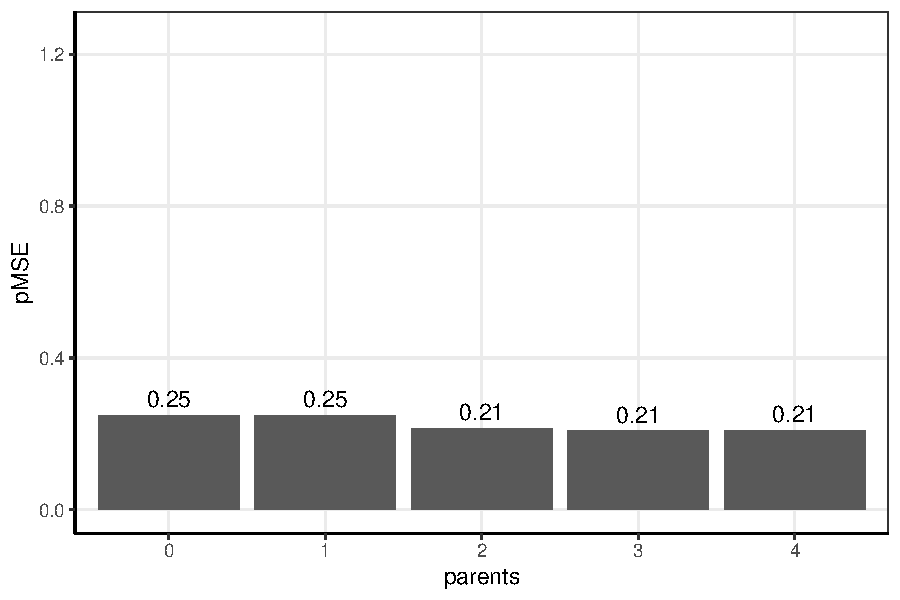
\includegraphics[width=\linewidth]{../graphs/datasynthesizer/datasynthesizer_fidelity_optimize_dataset_parents.pdf}
  \label{fig:tuning_ds_dataset}
\end{figure}

\begin{figure}[ht]
  \caption{Datasynthesizer two-way correlation  (pMSE)}
  \label{fig:ds_fidelity_two_way}
  \centering

  \begin{subfigure}{0.75\textwidth}
    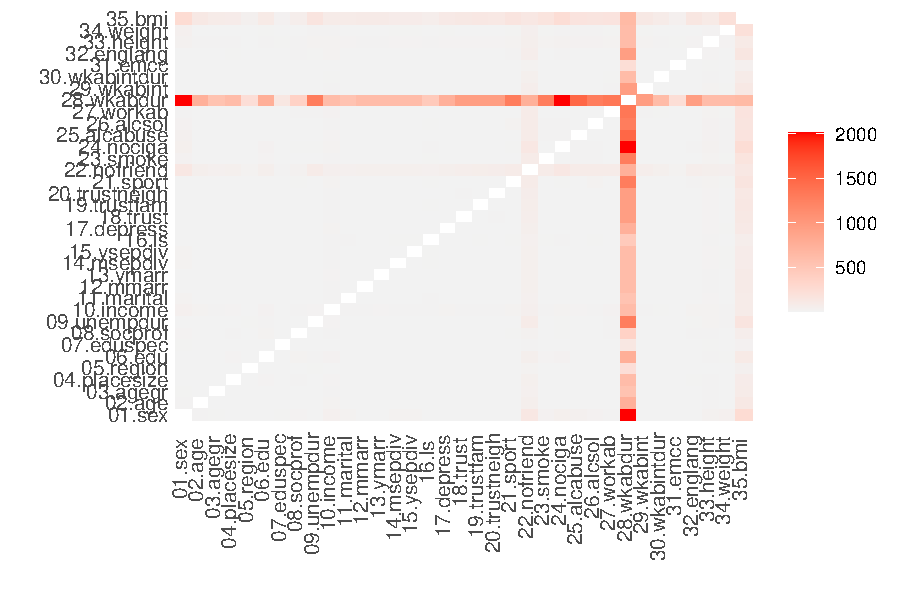
\includegraphics[width=\linewidth]{../graphs/datasynthesizer/datasynthesizer_fidelity_twoway_sd2011.pdf}
    \caption{SD2011(a)}
    \label{subfig:ds_fidelity_two_way_subfig-a}
  \end{subfigure}

  \begin{subfigure}{0.75\textwidth}
    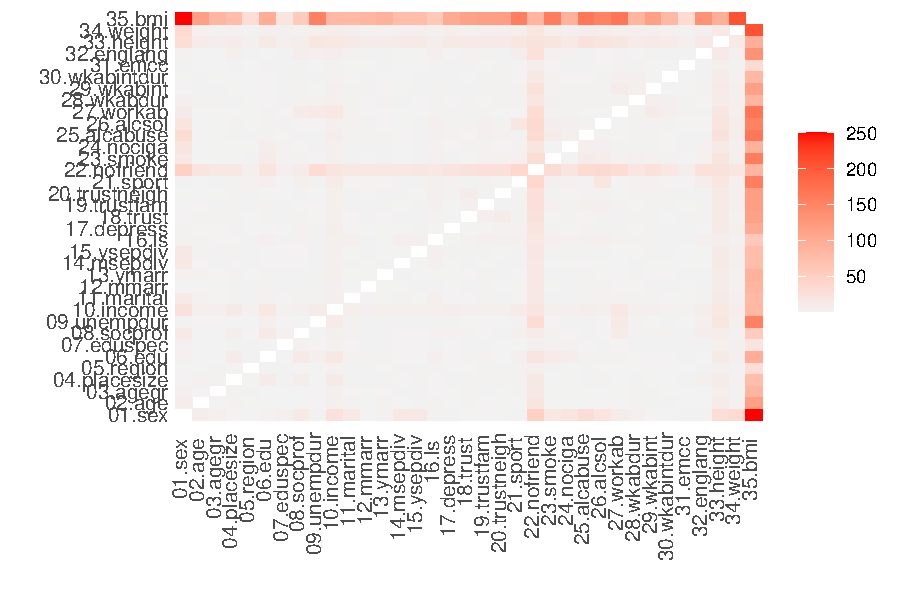
\includegraphics[width=\linewidth]{../graphs/datasynthesizer/datasynthesizer_fidelity_twoway_sd2011_clean.pdf}
    \caption{SD2011(b)}
    \label{subfig:ds_fidelity_two_way_subfig-b}
  \end{subfigure}

  \begin{subfigure}{0.75\textwidth}
    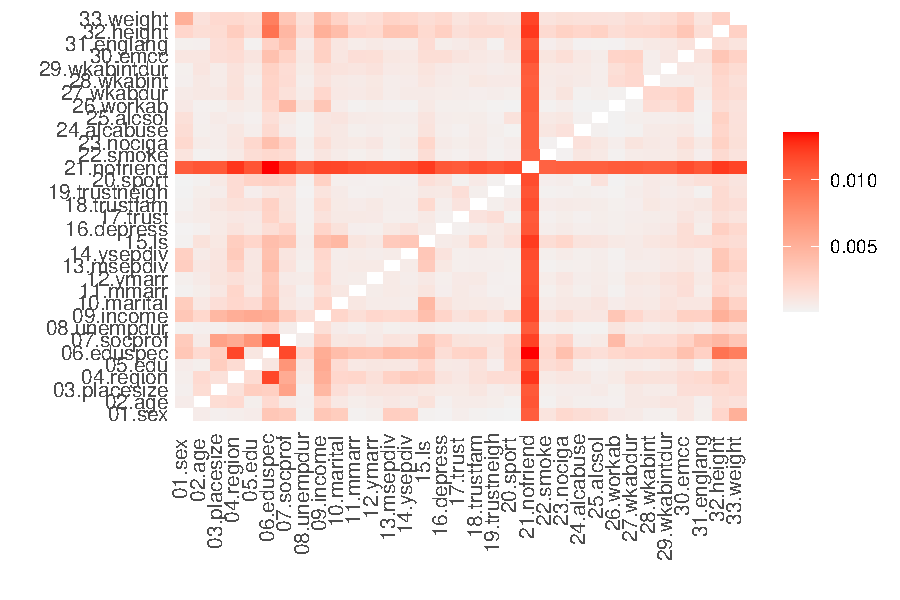
\includegraphics[width=\linewidth]{../graphs/datasynthesizer/datasynthesizer_fidelity_twoway_sd2011_clean_small.pdf}
    \caption{SD2011(c)}
    \label{subfig:ds_fidelity_two_way_subfig-c}
  \end{subfigure}
\end{figure}

\begin{figure}[ht]
  \caption{Frequency values for original and synthetic data (DataSynthesizer)}
  \label{fig:ds_variables}
  \centering

\begin{subfigure}{\textwidth}
    \caption{Variable: \texttt{wkabdur} (Work abroad duration)}
    \resizebox{\textwidth}{!}{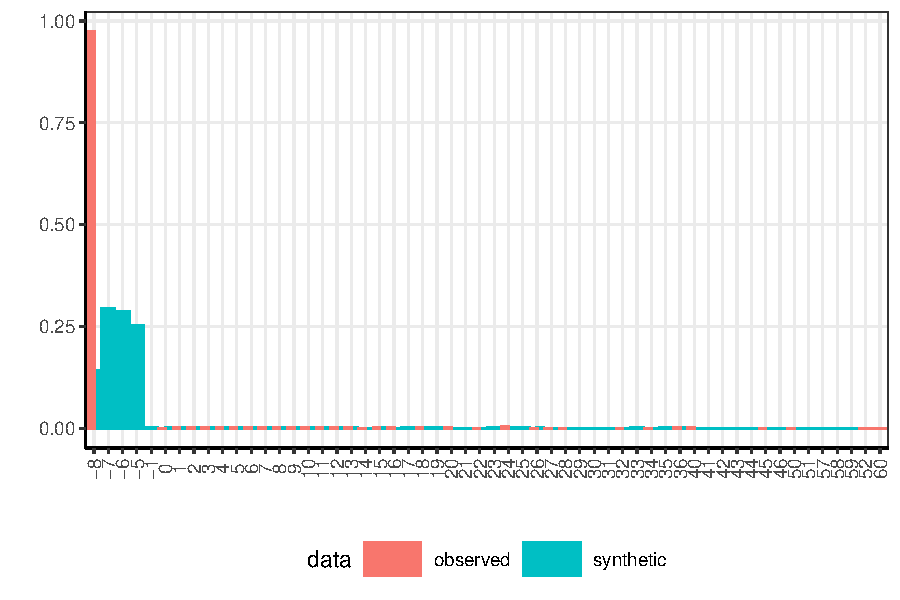
\includegraphics{../graphs/datasynthesizer/datasynthesizer_wkabdur.pdf}}
    \label{subfig:ds_variable_wkabdur}
\end{subfigure}

\begin{subfigure}{\textwidth}
    \caption{Variable: \texttt{bmi} (Body mass index)}
    \resizebox{\textwidth}{!}{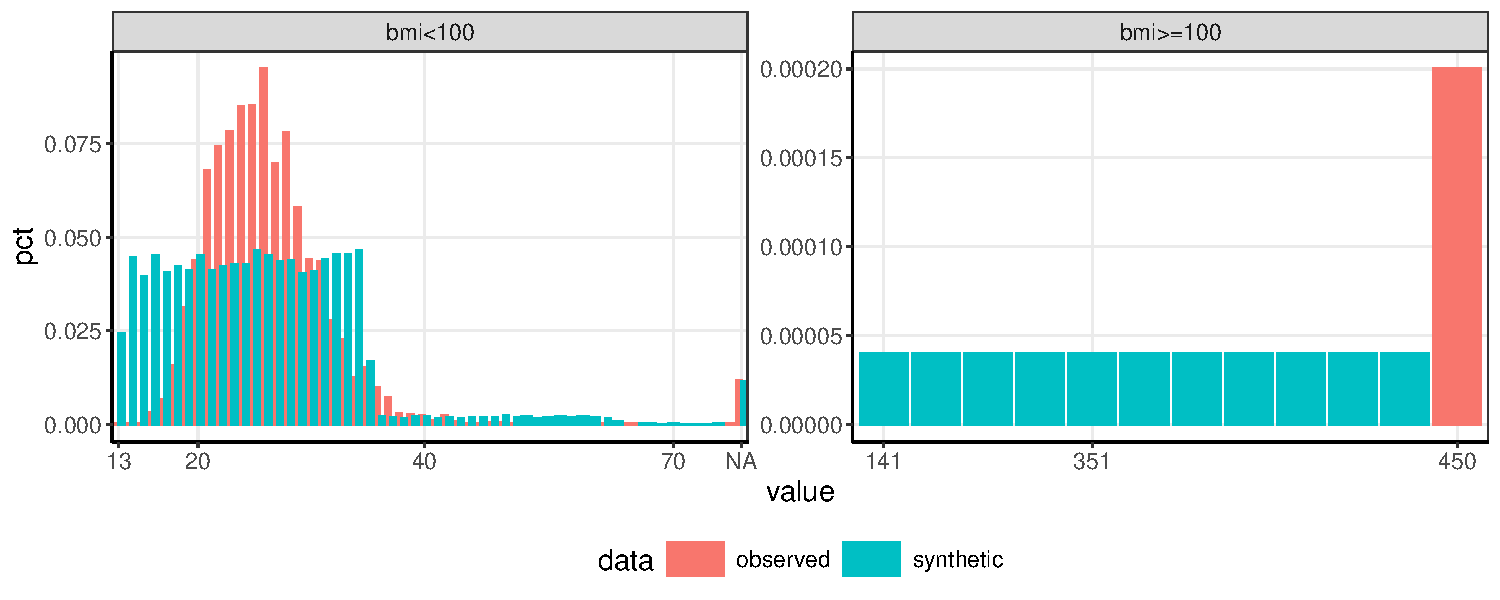
\includegraphics{../graphs/datasynthesizer/datasynthesizer_bmi.pdf}}
    \label{subfig:ds_variable_bmi}
\end{subfigure}


\begin{subfigure}{\textwidth}
    \caption{Variable: \texttt{nofriend} (Number of friends)}
    \resizebox{\textwidth}{!}{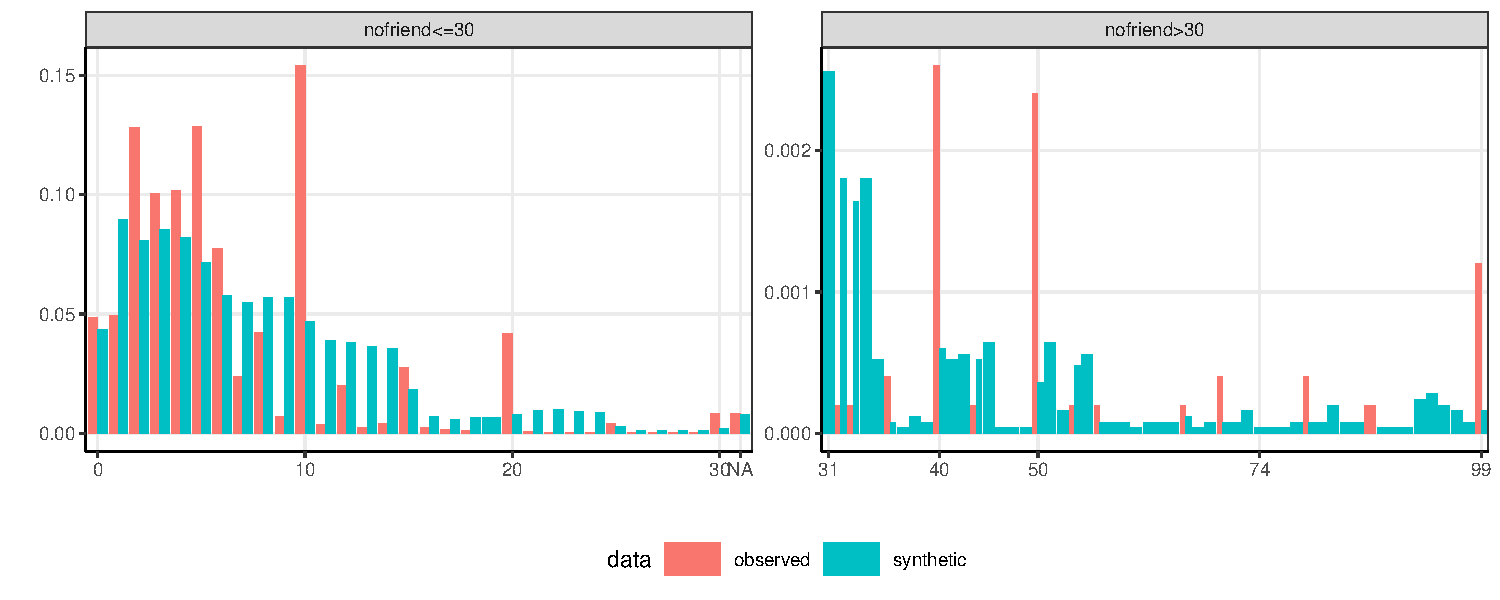
\includegraphics{../graphs/datasynthesizer/datasynthesizer_nofriend.pdf}}
    \label{subfig:ds_variable_nofriend}
\end{subfigure}
\end{figure}

\begin{figure}[ht]
  \caption{Tuning DataSynthesizer across data sets (parents = 2)}
  \label{fig:tuning_ds}
  \centering
  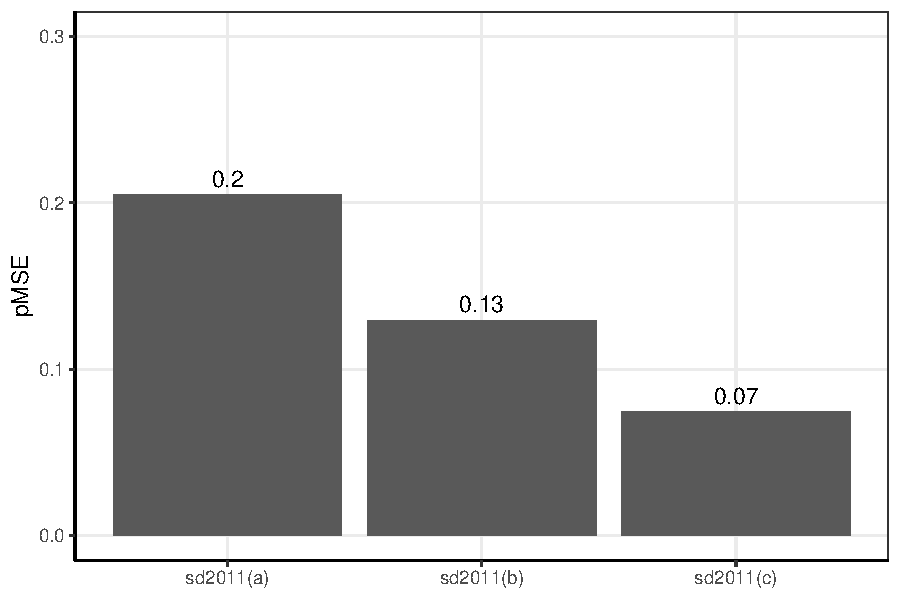
\includegraphics[width=\linewidth]{../graphs/datasynthesizer/datasynthesizer_fidelity_optimize_dataset_compare.pdf}
  \label{fig:tuning_ds_optimize_dataset_compare}
\end{figure}


%%%%%%%%%%%%%%%%%%%%%%%%%%%%%%%%%%%%%%
% Appendix
% CTGAN
%%%%%%%%%%%%%%%%%%%%%%%%%%%%%%%%%%%%%%
\clearpage
\section{Appendix: CTGAN}\label{appendix:CTGAN}
\setcounter{figure}{0}    
\setcounter{table}{0}    
\renewcommand*\thetable{\Alph{section}.\arabic{table}}
\renewcommand*\thefigure{\Alph{section}.\arabic{figure}}
\renewcommand{\theHfigure}{\Alph{section}.\arabic{table}}
\renewcommand{\theHtable}{\Alph{section}.\arabic{figure}}

\begin{table}[!h]
    \rowcolors{1}{white}{lightgray}
    \caption{Batch size and epochs = total steps}
    \centering
    \begin{tabular}{cllll>{\cellcolor{white}}p{1in}}
    % {cllllp{1in}}
    \toprule
    N & Batch size & Steps per Epoch & Epochs & Total Steps & Compare \\
    \midrule
    5.000 & 500 & 10 & 100 & 1,000 & \multirow{4}{1in}{Constant batch size, as shown in figure \ref{subfig:ctgan_fidelity_optimize_batch_size}}\\
    5.000 & 500 & 10 & 300 & 3,000 \\
    5.000 & 500 & 10 & 600 & 6,000 \\
    5.000 & 500 & 10 & 900 & 9,000 \\ \hline
    5.000 & 100 & 50 & 60 & 3,000  & \multirow{4}{1in}{Constant batch size, as shown in figure \ref{subfig:ctgan_fidelity_optimize_epochs}} \\
    5.000 & 250 & 20 & 150 & 3,000 \\
    5.000 & 500 & 10 & 300 & 3,000 \\
    5.000 & 1.000 & 5 & 600 & 3,000 \\ 
    \bottomrule
    \end{tabular}
\end{table}

\begin{figure}[ht]
  \caption{Tuning CTGAN (effect of steps)}
  \label{fig:ctgan_fidelity_optimize}
  \centering

  \begin{subfigure}{0.75\textwidth}
  \caption{Effect of batch size with constant steps (3.000)}
  \resizebox{\textwidth}{!}{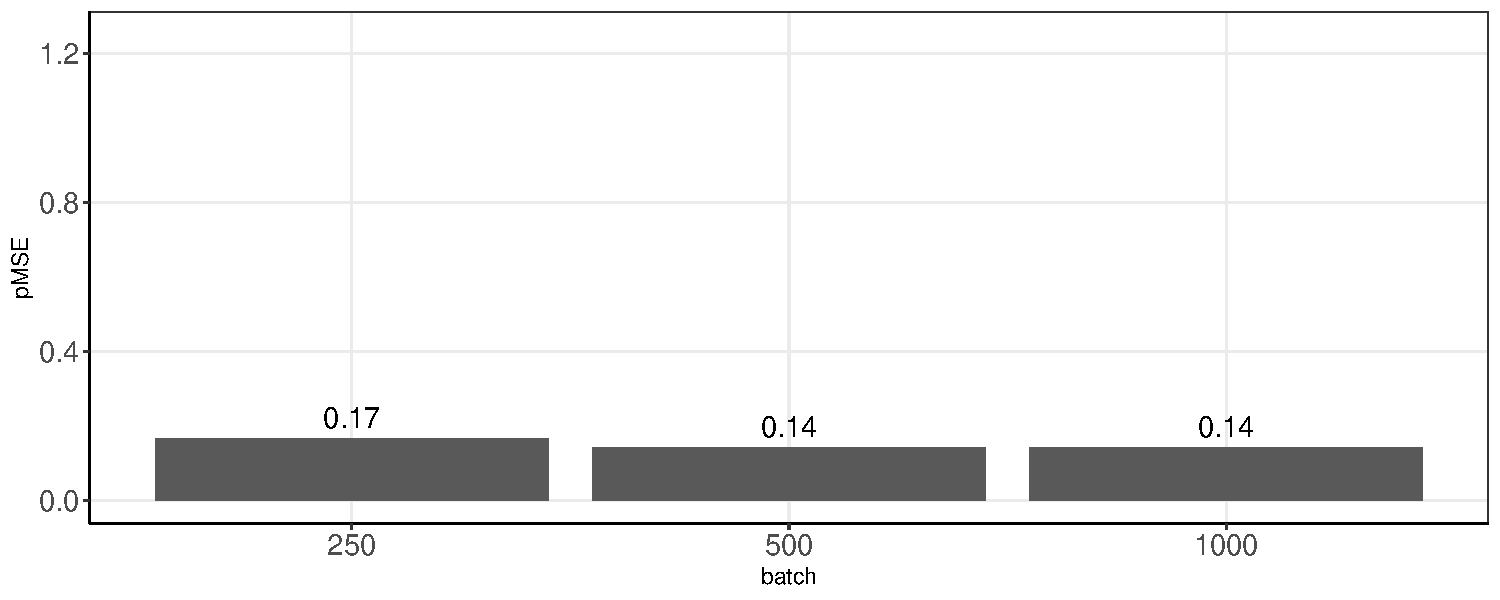
\includegraphics{../../ctgan/graphs/ctgan/ctgan_fidelity_optimize_batch_size.pdf}}
  \label{subfig:ctgan_fidelity_optimize_batch_size}
  \end{subfigure}

  \begin{subfigure}{0.75\textwidth}
  \caption{Effect of epoch number with constant batch size (500)}
  \resizebox{\textwidth}{!}{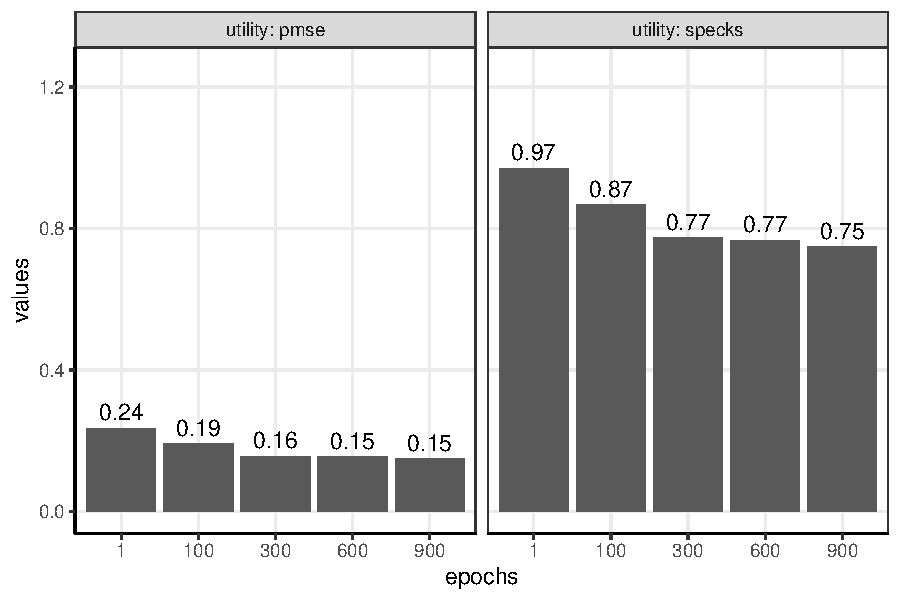
\includegraphics{../../ctgan/graphs/ctgan/ctgan_fidelity_optimize_epochs.pdf}}
  \label{subfig:ctgan_fidelity_optimize_epochs}
  \end{subfigure}

  \begin{subfigure}{0.75\textwidth}
    \caption{Effect of dimensionality}
      \resizebox{\textwidth}{!}{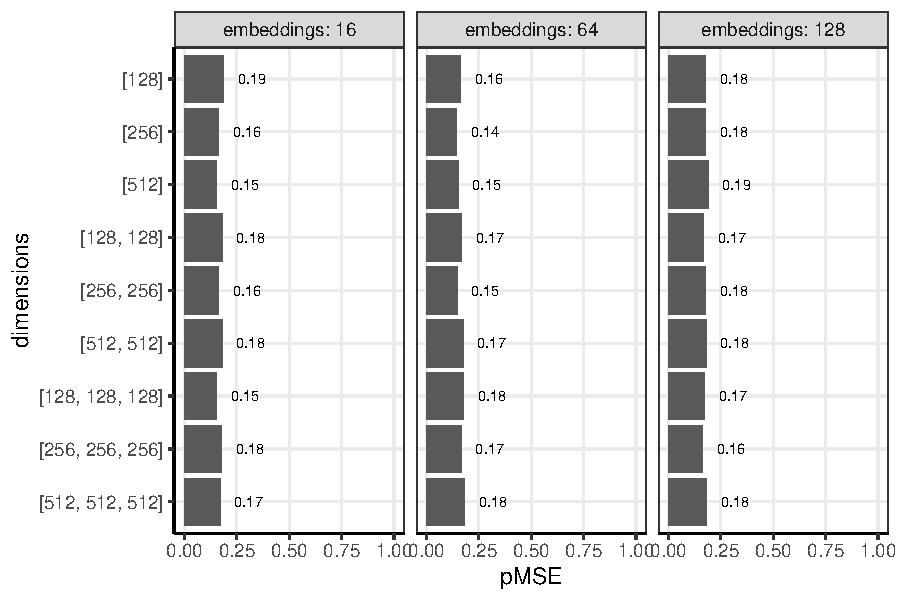
\includegraphics{../../ctgan/graphs/ctgan/ctgan_fidelity_optimize_dimensions.pdf}}
      \label{subfig:ctgan_fidelity_optimize_dimensions}
  \end{subfigure}
\end{figure}


\begin{figure}[ht]
  \caption{CTGAN two-way correlation (pMSE)}
  \label{fig:ctgan_fidelity_two_way}
  \centering

  \begin{subfigure}{0.75\textwidth}
    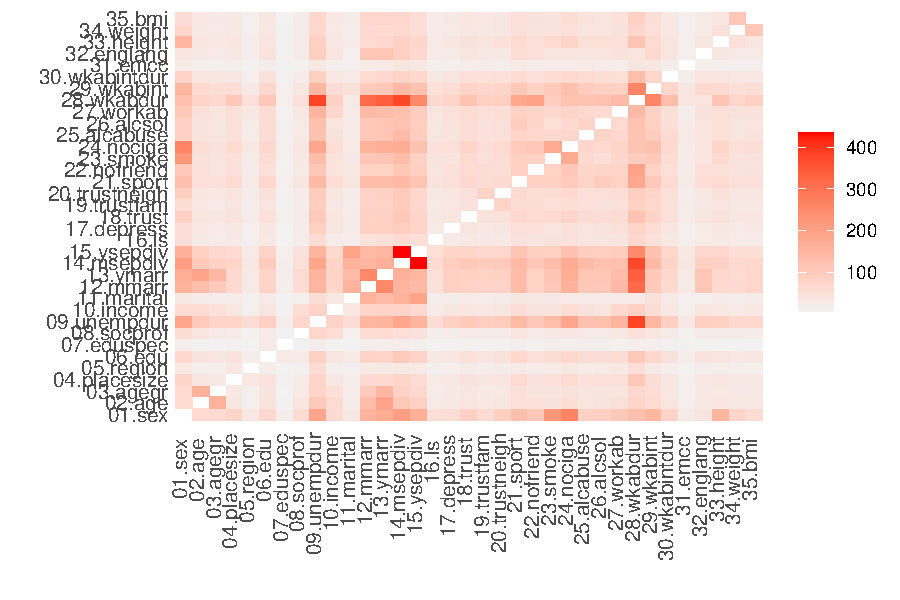
\includegraphics[width=\linewidth]{../graphs/ctgan/ctgan_fidelity_twoway_sd2011.pdf}
    \caption{SD2011(a)}
    \label{fig:ctgan_fidelity_two_way_subfig-a}
  \end{subfigure}

  \begin{subfigure}{0.75\textwidth}
    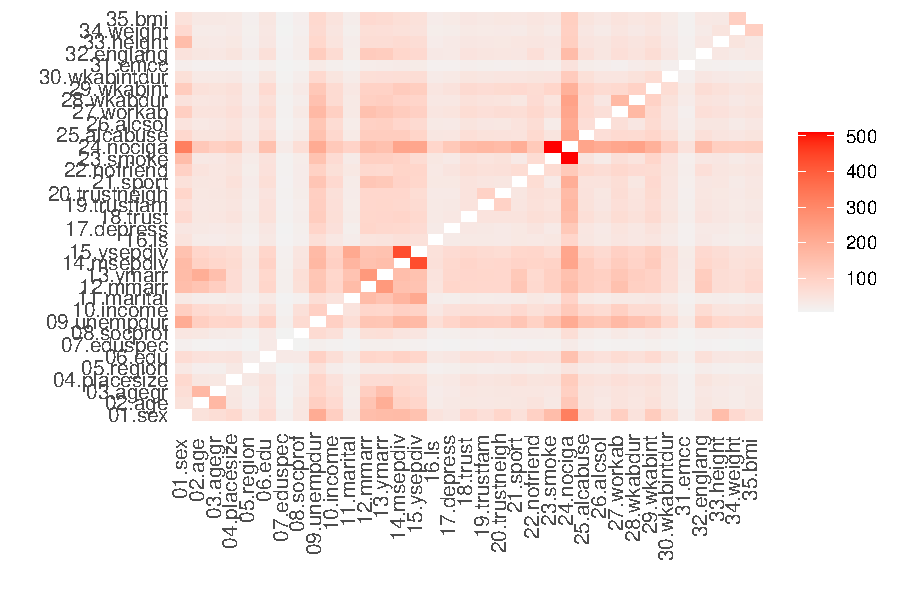
\includegraphics[width=\linewidth]{../graphs/ctgan/ctgan_fidelity_twoway_sd2011_clean.pdf}
    \caption{SD2011(b)}
    \label{fig:ctgan_fidelity_two_way_subfig-b}
  \end{subfigure}

  \begin{subfigure}{0.75\textwidth}
    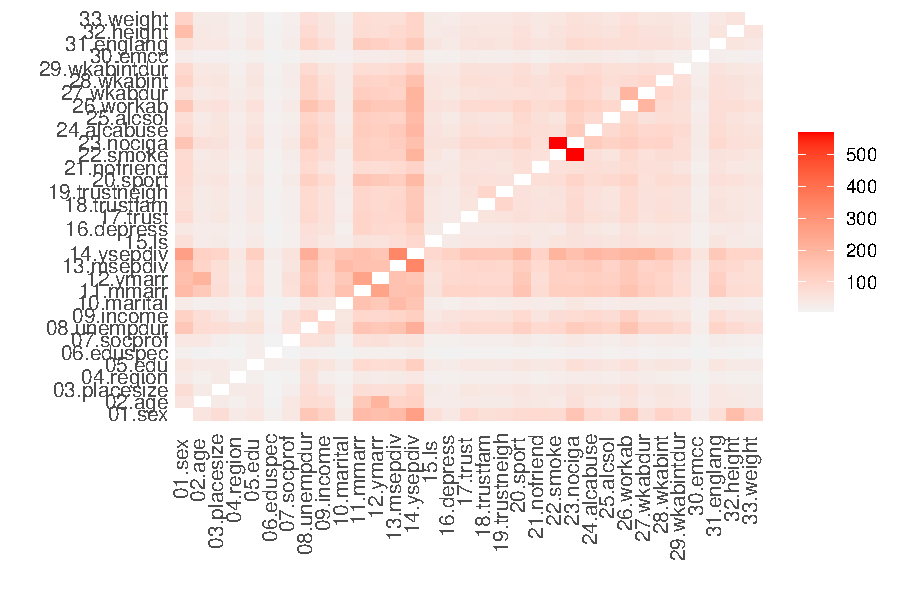
\includegraphics[width=\linewidth]{../graphs/ctgan/ctgan_fidelity_twoway_sd2011_clean_small.pdf}
    \caption{SD2011(c)}
    \label{fig:ctgan_fidelity_two_way_subfig-c}
  \end{subfigure}

\end{figure}

%%%%%%%%%%%%%%%%%%%%%%%%%%%%%%%%%%%%%%
%%%%%%%%%%%%%%%%%%%%%%%%%%%%%%%%%%%%%%
%SYNTHPOP
%%%%%%%%%%%%%%%%%%%%%%%%%%%%%%%%%%%%%%
%%%%%%%%%%%%%%%%%%%%%%%%%%%%%%%%%%%%%%
\begin{figure}[ht]
  \caption{Synthpop two-way correlation  (pMSE)}
  \label{fig:synthpop_fidelity_two_way}
  \centering

  \begin{subfigure}{0.75\textwidth}
    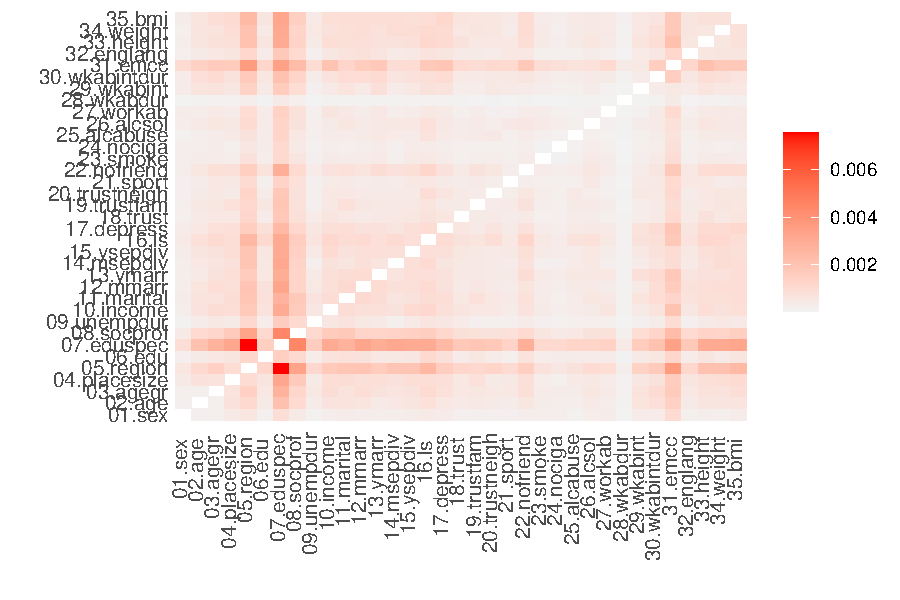
\includegraphics[width=\linewidth]{../graphs/synthpop/synthpop_fidelity_twoway_sd2011.pdf}
    \caption{SD2011(a)}
    \label{fig:synthpop_fidelity_two_way_subfig-a}
  \end{subfigure}

  \begin{subfigure}{0.75\textwidth}
    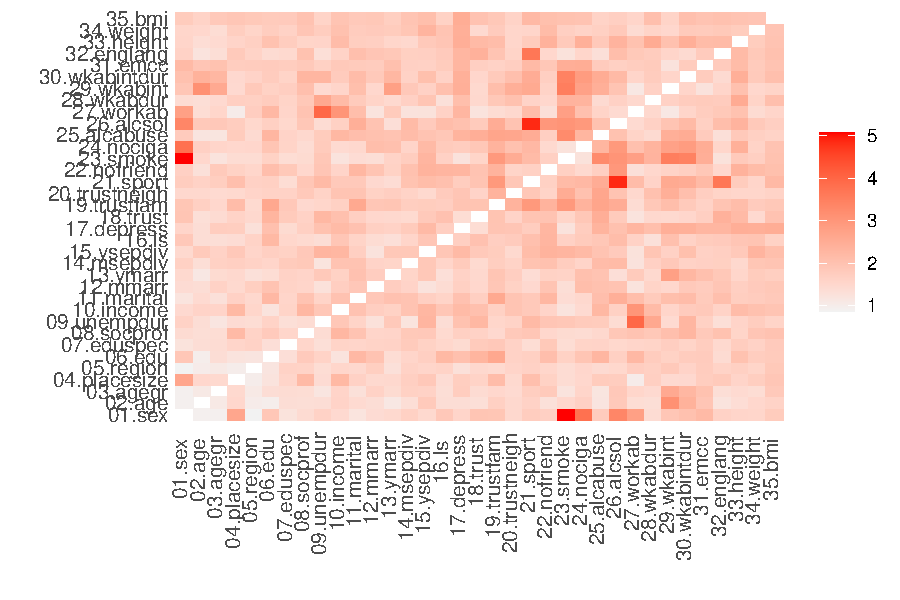
\includegraphics[width=\linewidth]{../graphs/synthpop/synthpop_fidelity_twoway_sd2011_clean.pdf}
    \caption{SD2011(b)}
    \label{fig:synthpop_fidelity_two_way_subfig-b}
  \end{subfigure}

  \begin{subfigure}{0.75\textwidth}
    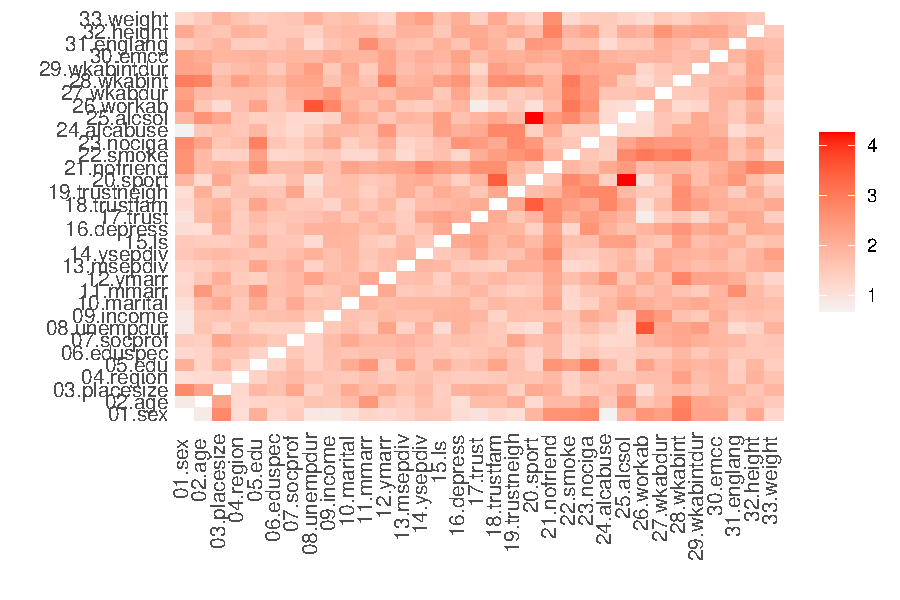
\includegraphics[width=\linewidth]{../graphs/synthpop/synthpop_fidelity_twoway_sd2011_clean_small.pdf}
    \caption{SD2011(c)}
    \label{fig:synthpop_fidelity_two_way_subfig-c}
  \end{subfigure}

\end{figure}

